%!TEX root = ../../super_main.tex

\section{Sensor Providers}
\label{sec:sensor_providers}

We have implemented a threaded abstraction over the different data sources that the system should utilize in order to gather context for the labels that will eventually be combined to form the output training data for the system. The abstraction is threaded because we want the Android application to be able to gather information from multiple sources concurrently. This is done in order to make sure that the gathered data is obtained temporally close to when the label for the data was obtained. 

\subsection{Temporality}

% Det bliver hurtigt til meget data når man arbejder med continious data
% Vi bruger sample frequency til at lave mellemrum mellem samples i tid fordi det ikke er så brugbart at have 8gb data for et minuts målinger
% Vi vil gerne have flere measurements per sample så vi kan undgå upræcise målinger

As described in \secref{sec:availability_of_data_sources}, some data sources are continuous. This effectively means that it would become infeasible to store this data due to many factors including excessive battery drain, file size etc\todo{We need to research if file size is actually a problem}. Furthermore, it might not be relevant to store a huge amount of measurements for a small time period.

\begin{figure}[!htbp]
    \centering
    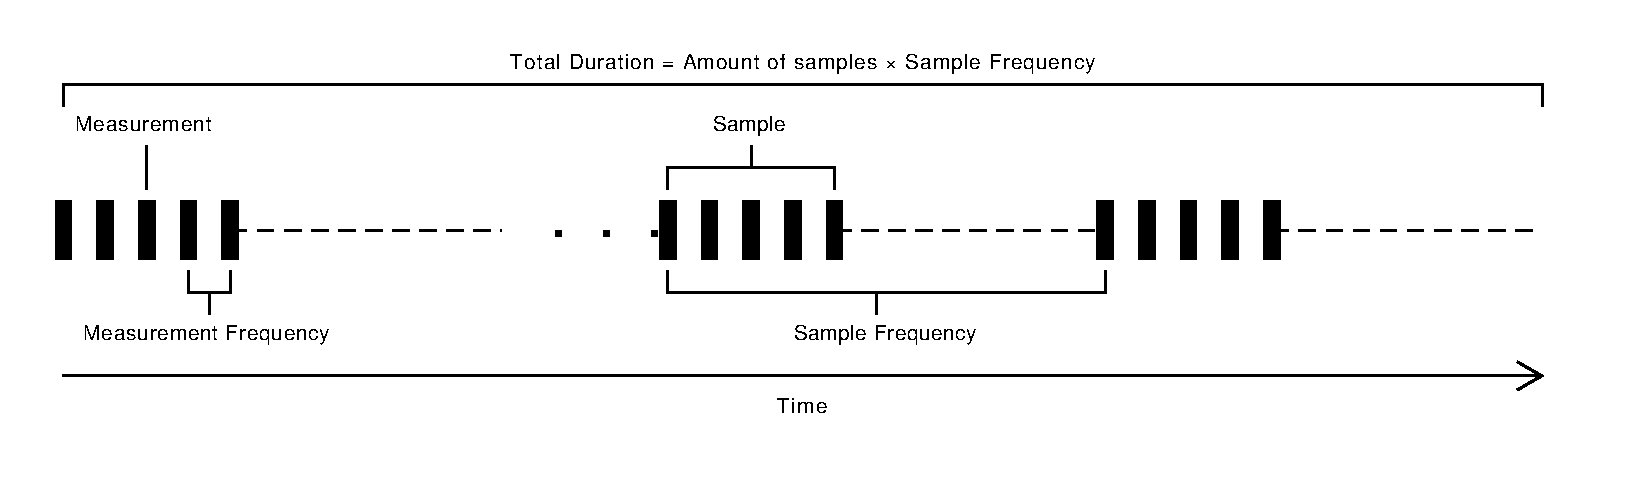
\includegraphics[width=\textwidth]{unsorted/sample_temporality}
    \caption{Overview of sample and measurement temporality.}
    \label{fig:sample_temporality}
\end{figure}

\subsection{Implementation}

% Future<T> Objects
% 

% \lstinputlisting[
%    style = java,
%    caption = {Property similarity on a component.},
%    label = {lst:attribute_difference},
%]{content/implementation/annotation/attribute_difference.java}